\documentclass[12pt,english,twoside]{article}

\usepackage[utf8]{inputenc}
\usepackage[T1]{fontenc}

\usepackage[letterpaper, margin=2cm]{geometry}
\usepackage{color}
\usepackage{graphicx}
\usepackage{times}
\usepackage{etoolbox}
\usepackage{fancyhdr}
\usepackage{enumitem}
\usepackage{indentfirst}       % indent the first line of the section and subsection
\usepackage{titlesec}          % customizing the section titles
\usepackage{hyperref}
\usepackage{babel}


\usepackage{amssymb}
\usepackage{amsmath}
\usepackage{fancybox}
\usepackage{xfrac}	% fraction de type "1/4"
\usepackage{cases}	% système équation
\usepackage[overload]{empheq}
\usepackage{bm}		% pour mettre en gras .
\usepackage{units} 	% x/y barre latérale pour les fractions

\usepackage{caption}
\usepackage{subcaption}

\pagestyle{fancy}			        % set default page style 
\setlength{\parskip}{0pt}
\setlist{nolistsep}

% custom \thebibliography environment
\makeatletter
\renewcommand*{\@biblabel}[1]{\hfill#1.}
\makeatother

% formatting the head rule and the foot rule
\makeatletter
\patchcmd{\headrule}{\hrule}{\color{blue}\hrule}{}{}
\patchcmd{\footrule}{\hrule}{\color{blue}\hrule}{}{}
\makeatother

% set first page erase the head rule in the first page
\fancypagestyle{firstpage}{
\fancyhead{}
\fancyfoot{}
\fancyfoot[LE,RO]{\small \thepage}
\renewcommand{\headrulewidth}{0pt}
\renewcommand{\footrulewidth}{1.5pt}
}

% custom \maketitle environment
\makeatletter 
\def\maketitle{ 
  \thispagestyle{firstpage} 
\noindent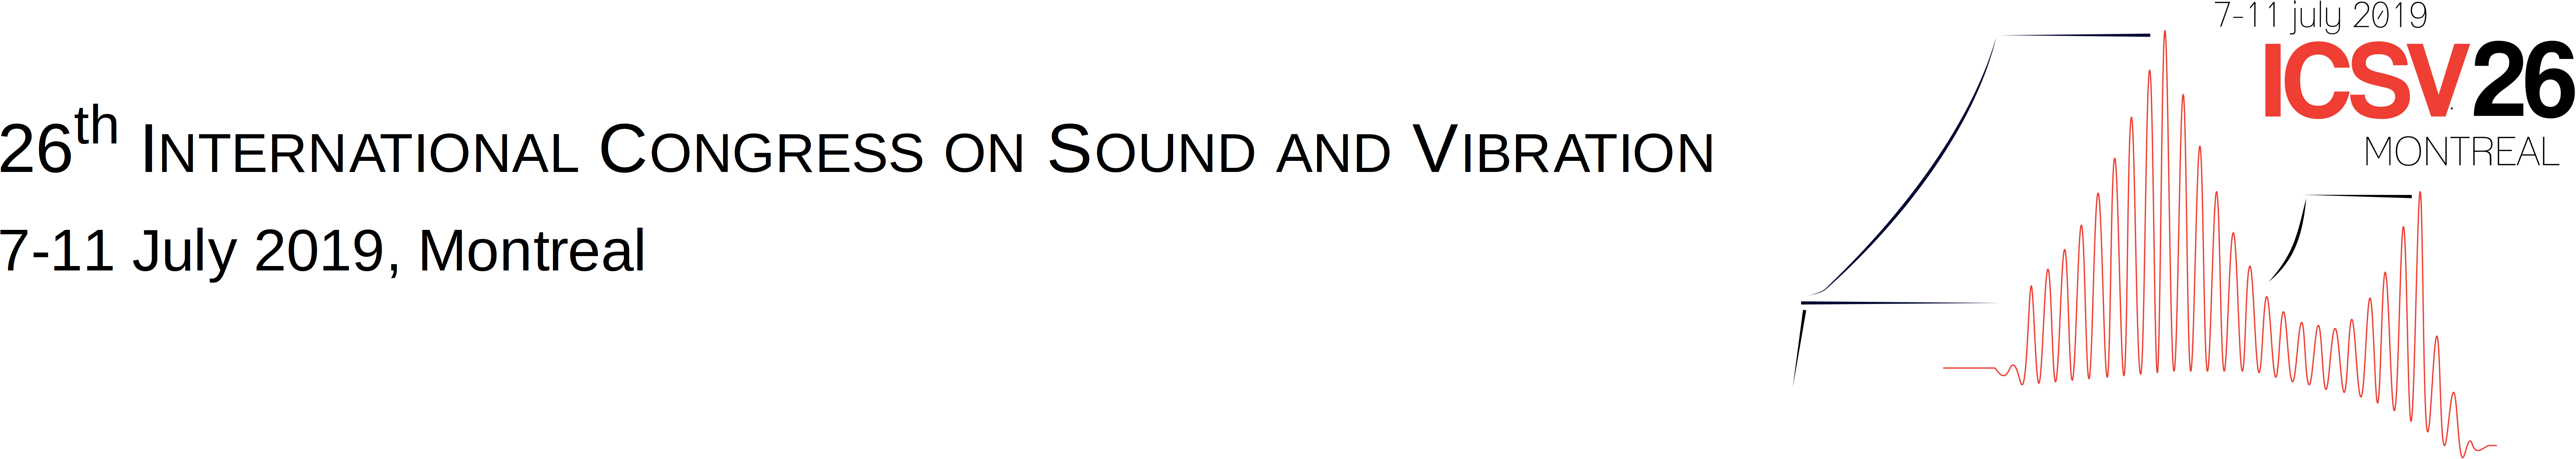
\includegraphics[width=\textwidth]{ICSV26-header.png}\\
  {
   \fontsize{17}{20}\selectfont\sffamily{}  \noindent \MakeUppercase{\textbf{\@title}}
  
   \bigskip
   \fontsize{14}{20}\selectfont\rmfamily{} \noindent \@author
  } 
} 
\makeatother 

% setting the standard headers and footers
\fancyhead{}
\fancyfoot{}
\fancyhead[LE,RO]{\small ICSV26, Montreal, 7-11 July 2019}
\fancyfoot[RE,LO]{\small ICSV26, Montreal, 7-11 July 2019}
\fancyfoot[LE,RO]{\small \thepage}
\renewcommand{\headrulewidth}{1.5pt}
\renewcommand{\footrulewidth}{1.5pt}

%custom section appearance
\titleformat{\section}
  {\fontsize{14}{14}\normalfont\sffamily\bfseries}
  {\thesection.}{1em}{}                % insert a point after the section number like the original .doc file

\titleformat{\subsection}
  {\normalfont\sffamily\bfseries}
  {\thesubsection}{1em}{} 

\titleformat{\subsubsection}
  {\normalfont\sffamily\small}
  {\textit{\thesubsubsection}}{1em}\textit{{}}


%%%%%%%%%%%%%%%%%%%%%%%%%%%%%%%%%%%%%%%%%%%%%%%%%%%%


%%% PLEASE INSERT PAPER TITLE HERE
\title{Study of the Non-negative Matrix Factorization behavior to estimate the urban traffic sound levels}

%%% PLEASE INSERT AUTHOR AND AFFILIATIONS HERE
\author{
Jean-R\'emy Gloaguen, {\small \textit{UMRAE, CEREMA, France, email: jean-remy.gloaguen@orange.fr}}
\medskip
\\
Mathieu Lagrange, {\small \textit{LS2N, Ecole Centrale de Nantes, France}}
\medskip
\\
Arnaud Can, {\small \textit{UMRAE, Ifsttar, France}}
\medskip
\\
\emph{and} Jean-Fran\c cois Petiot, 
{\small \textit{LS2N, Ecole Centrale de Nantes, France}}}



\begin{document}


\maketitle

\renewcommand{\abstractname}{\vspace{-\baselineskip}} % erase the space between authors and abstract

\begin{abstract}	\noindent
The advent of low-cost acoustic sensor networks in cities raises new interesting approaches for improving the monitoring of the acoustic quality of cities. Many innovative approaches are developed to improve knowledge on sound environments: sound environment recognition, sound source detection, etc. In order to improve the road traffic noise mapping, the use of a specific version of the Non-negative Matrix Factorisation (NMF), named thresholded initialized NMF, as a source separation method to estimate the sound level of road traffic from measurements, has proved to be a successful approach.
This paper proposes to further detail the functioning of the thresholded initialized NMF on a corpus composed of urban sound scenes mixing traffic and specific interfering components with calibrated sound levels in order to better understand its behavior according to the different sources encountered.
The study reveals the different performances of this approach depending on the noise levels of the interfering sources and their proximity to the urban traffic spectrum.\\

\noindent Keywords: road traffic, non-negative matrix factorization, traffic noise mapping
\end{abstract}

\quad\rule{425pt}{0.4pt}


\section{Introduction} 
%----------------------------------------------------------------------------------------------

Low-cost acoustic sensor networks are currently deployed in cities to assess the urban sound environment as the DYNAMAP project \cite{dynamap_2016} in Italy or the CENSE project \cite{picaut2017characterization} in France. The use of such networks allows innovative approaches to better estimate the soundscape through, for instance, the urban sound environment classification \cite{maijala2018environmental}. One application of interest is the improvement of the traffic noise mapping ordered by the European Directive 2002/EC/49. These maps are currently generated from predictive models and collected traffic data to estimate the A-weighting traffic sound level through the day, $L_{DEN}$, and the night, $L_N$. The use of these networks could facilitate the updating of the traffic maps or even the generation of dynamic maps by the assimilation of the measured data with the predicted sound levels \cite{ventura2018assimilation}. 
Prior to data assimilation, the issue is to correctly estimate the traffic sound level from acoustic measurements \cite{leiba2017large,socoro2017anomalous}. As the urban sound environment is a complex environment gathering lots of different sounds (car passages, voices, whistling bird, car horn, airplanes, etc.) that overlap, the estimation of the traffic sound level  based on acoustic measurements is not a trivial task \cite{mesaros_sound_2015}. Although near major roads, traffic is predominant, there are many places where it overlaps with other sound sources that contribute significantly to the overall sound levels. To circumvent this issue, Socor\'o et al. propose an Anomalous Noise Events Detector \cite{socoro2017anomalous}. It consists in detecting in each time frame the unwanted sound sources from labeled recordings, \textit{i.e.} that are not related to the traffic component. Those are then discarded in order not to take them into account during the estimation of the traffic sound level.
An alternative approach has been proposed in Gloaguen et al. \cite{gloaguen2019road}, which is based on the blind source separation paradigm to reliably estimate the traffic noise level. 
It consists in separating the contribution of the traffic from the other sources within a polyphonic scene with the help of the Non-negative Matrix Factorization framework (NMF). 
In their study, the authors present a new approach of this method, named thresholded initialized NMF (TI NMF) whose performances to  estimate the traffic sound level exceed those of existing approaches (supervised and semi-supervised). TI NMF then makes it possible to determine the noise level with an estimation error less than 2 dB\footnote{Tool available at: \url{https://bitbucket.org/jean-remy_g/trafficsoundlevelestimation}}. 
To do so, their study is based on simulated sound mixtures covering different sound environments (park, quiet street, noisy street, very noisy street) whose realism has been tested on a perceptual test to ensure that the sound mixtures are similar to audio recorded in the streets \cite{gloaguen2017creation}. 
One major advantage of this approach is its application in a wide range of urban areas, even where the traffic noise is relatively low compared to the remaining contributions. In addition, NMF is perfectly suited for monaural sensor networks. 
Here, to better understand the TI NMF behavior, this method is tested on a new corpus of sound mixtures mixing a traffic component with a calibrated sound level and specific sound classes. The use of simulated sound scenes allows rigorous experimental validation as it offers a high level of control on the design of the scenes and the knowledge of the exact contribution of the traffic component ($L_{p,traffic}$).
The remaining of the paper is organized as follows. Section \ref{part:nmf} details the technical aspects of TI NMF. Section \ref{part:protocol} describes the urban sound mixtures and the experimental protocol setup. Section \ref{part:results} presents and discusses the outcomes of the numerical results.

\section{Non-negative Matrix Factorization}\label{part:nmf}
\subsection{Description of NMF}

Non-negative Matrix Factorization is a linear approximation method introduced by Lee and Seung, \cite{lee_learning_1999}, which can be used to approximate the spectrogram $\mathbf{\tilde{V}}$ (obtained using a Short-Term Fourier Transform) of an audio file, $\mathbf{V}$, $\in \mathbb{R}^+_{F \times N}$ as $\mathbf{V} \approx \mathbf{\tilde{V}} = \mathbf{WH}$
where $\mathbf{W} \in \mathbb{R}^+_{F \times K}$ is the \textit{dictionary} (or basis) matrix composed of audio spectra and $\mathbf{H} \in \mathbb{R}^+_{K \times N}$ is the \textit{activation} matrix, which summarizes the temporal evolution of each element of $\mathbf{W}$. As the constraint of non-negativity of $\mathbf{W}$ and $\mathbf{H}$ is considered, NMF allows only additive combinations between the element of $\mathbf{W}$, thus inducing a part-based representation.
The choice of the dimensions is often made so that $F\times K + K \times N < F \times N$ \cite{fevotte_nonnegative_2009}. NMF is then considered as a low rank approximation method. However, this constraint is not mandatory. To estimate the quality of the approximation, an objective function is minimized

\begin{equation}\label{eq:min-D-WH}
\underset{\mathbf{H} \geq 0, \mathbf{W} \geq 0}{\min} D\left(\mathbf{V} \vert \vert \mathbf{\tilde{V}}\right) = \sum_{f = 1}^{F} \sum_{n = 1}^{N} d_{\beta}
\left(\textbf{V}_{fn} \vert \left[ \textbf{WH} \right]_{fn} \right).
\end{equation}

The operator $d_{\beta}(x\vert y)$ is a divergence calculation and usually belongs to the $\beta-$divergence class \cite{fevotte_nonnegative_2009} in which the well known Euclidean distance and the Kullback-Leibler divergence.

\subsection{Thresholded initialized NMF}
Thresholded initialized NMF has been proposed in \cite{gloaguen2019road} and is based on the unsupervised NMF. Usually in unsupervised learning, $\mathbf{W}$, as  $\mathbf{H}$, is initialized randomly. In TI NMF, an initial dictionary, $\mathbf{W_0}$ dedicated to a specific sound source, is built from a learning database (see part \ref{part:test_datase}).
Then NMF is performed where $\mathbf{W}$ and $\mathbf{H}$ are updated alternatively. $\mathbf{W}$ is therefore updated with a forced initialization with \textit{a priori} knowledge but is adapted to the actual content of the scene under study. Among the different algorithms proposed to solve \ref{eq:min-D-WH}, the multiplicative update of $\mathbf{W}$ and $\mathbf{H}$ is chosen as it has been well studied in the literature and ensures convergence of the results. It can be found in \cite{fevotte_algorithms_2011}.
After $N$ iterations, a measure of similarity $D\left(\mathbf{W_0} \vert \vert \mathbf{W}^{'} \right)$ between $\mathbf{W_0}$ and the obtained dictionary $\mathbf{W}^{'}$ for each element $k$ is computed using a cosine similarity metric,

\begin{equation}
D\left(\mathbf{W_0}_k \vert \vert \mathbf{W}^{'}_k \right) = \frac{\mathbf{W_0}_k.\mathbf{W}^{'}_k}{\vert \vert \mathbf{W_0}_k  \vert \vert . \vert \vert \mathbf{W}^{'}_k \vert \vert}.
\end{equation}

$D\left(\mathbf{W_0}_k \vert \vert \mathbf{W}^{'}_k \right) = 1$ means that the $k$-th element of $\mathbf{W}^{'}$ is identical to the $k$-th element of $\mathbf{W_0}$. On the contrary, $D\left(\mathbf{W_0}_k \vert \vert \mathbf{W}^{'}_k \right)$ = 0 means that the elements are very different. This measure has the advantage to be bounded between 1 and 0 and to be invariant with respect to scale. The elements in $\mathbf{W}^{'}$ that can belong to $\mathbf{W}_{traffic}$ are selected by a \textit{hard thresholding} method. It is defined as $\mathbf{W}^{'}_k \in \mathbf{W}_{k,traffic}$ if $D\left(\mathbf{W_0}_k \vert \vert \mathbf{W}^{'}_{k} \right) > t$ where $t$ is a fixed threshold.

\section{Experimental protocol}\label{part:protocol}

In order to study the TI NMF behavior according urban sounds sources, the experimental protocol, the databases and the experimental factors involved in the experience are presented, each of these experimental factors having multiples modalities (see Figure \ref{fig:bloc_nmf}).  

\subsection{Test databases}\label{part:test_datase}

The test database is designed with the sound scene synthesizer \textit{SimScene} \footnote{Open-source project available at: \url{https://bitbucket.org/mlagrange/simScene}} \cite{rossignol_simscene_2015}, a simulator that creates monaural sound scenes by sequencing audio samples that come from an isolated sound database \cite{lagrange2015evaluation}. 
The database\footnote{available at: \url{https://zenodo.org/record/1213793}} used is presented in \cite{gloaguen2017creation}. This offers a controlled framework to design at low cost a wide diversity of sound environments in which all the traffic components are known, thus allowing the computation of the reference level.
This database is composed of 3 sub-corpus of 25 audio files each lasting 30 seconds. Each sub-corpus is characterized by an interfering sound class which are \textit{animals} (an.), composed of barking dogs and whistling birds, \textit{humans} (hu.), composed of crowd noises and voices, and \textit{transportation} (tr.), composed of train, tramway and plane sounds. Each sound mixture is summed  with a traffic component (the sum of the road traffic background noise and the sound events generated by the \textit{passing car} class) that makes the estimation of the traffic level more difficult. In each file, the traffic component is present. To test different scenarios, each audio file is duplicated with the traffic sound level of the entire sound scene, $L_{p,traffic}$, fixed to a calibrated level according to the sound level of the interfering class, $L_{p,interfering}$ such as $
TIR = L_{p,traffic}-L_{p,interfering}$ with the \textit{Traffic Interference Ratio} $TIR \in \lbrace$-12, -6, 0, 6, 12$\rbrace$ dB.
The range of these values is large but in the urban environments, the $TIR$ seems to be between -6 dB and 12 dB \cite{gloaguen2017creation}. The case $TIR$ = -12 dB is then an extreme case to study the NMF behavior. When $TIR < 0$ dB, the traffic component is less present than the interfering class. On the contrary, for $TIR > 0$ dB, the traffic class is louder than the interfering class. The total number of scenes in the test database is then 375 (3 sub-corpus $\times$ 25 scenes $\times$  5 $TIR$ values) leading to a full duration of 3 hours and 15 minutes.

\subsection{NMF experimental factors}

\begin{figure}
    \centering
    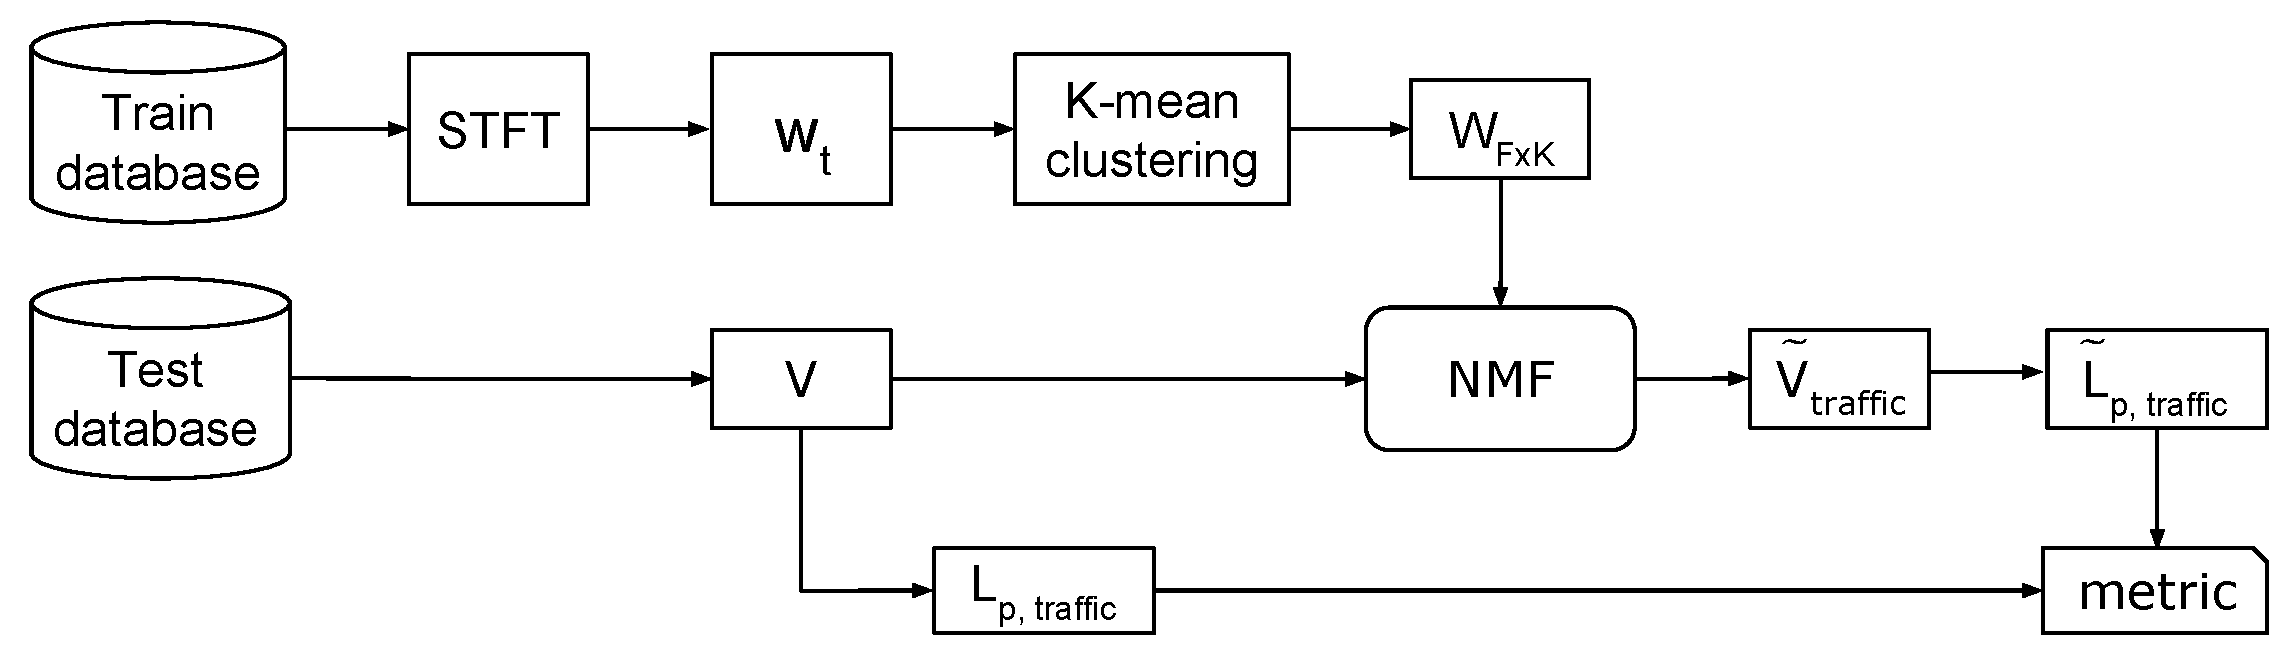
\includegraphics[width=.7\linewidth]{./figures/bloc_diagram_complet_NMF_EN.pdf}
    \caption{Block diagram of the NMF estimator with the dictionary design composed from a second sound database.}
    \label{fig:bloc_nmf}
\end{figure}

The Figure \ref{fig:bloc_nmf} presents the different steps involved in the NMF process. 
The dictionary design requires a train database composed of 53 audio samples of passing cars. A four-step process is realized to generate different versions of dictionaries with a sub-sampling of the audio spectrograms by a windowing of $w_t$ seconds ($w_t\in \lbrace 0.5,~1\rbrace$ second), a rms calculation of each window and a $K$-means clustering algorithm reducing the number of spectra to $K \in \lbrace$25, 50, 100, 200$\rbrace$. Each basis vector of $\mathbf{W}$ is normalized such as $\vert \vert \mathbf{W_k} \vert \vert = 1$ with $\vert \vert \bullet \vert\vert$ the $\ell$-1 norm. The 8 versions of the dictionary are then used as the initial dictionaries $\mathbf{W_0}$. A full description of the dictionary design can be found in \cite{gloaguen2019road}.
100 iterations are performed with the Euclidean distance and the Kullback-Leibler divergence. The spectrogram $\mathbf{V}$ and the dictionary $\mathbf{W}$ are expressed with third octave bands ($F$ = 29). This coarser method allows us to reduce the dimensionality and thus decrease the computation time. But, most of all, it is a suited representation to this sound environment as third octave bands are widely used in the urban acoustic field, compared to MFCCs for instance. The range of threshold values is set between 0 and 1 with a 0.01 increment step. Considering the experimental factors (sub-corpus, $TIR$, $w_t$, $K$, EUC dist./K-L div., $t$) derived from the different modalities of each experimental factor, 24240 settings are performed. For each setting, the estimator is performed on the 25 scenes of a sub-corpus. For one sound scene, the estimated traffic sound level, $\tilde{L}_{p,traffic}$, of the entire scene is calculated, $\tilde{L}_{p,traffic} = 20 \times \log_{10}\left(\frac{p_{rms}}{p_0}\right)$ where $p_{rms}$ is the effective pressure deducted from the estimated traffic spectrogram $\mathbf{\tilde{V}}_{traffic}$ and $p_0$ is the reference sound pressure, $p_0 = 2 \times 10^{-5} Pa$.  The $A$-weighting of the sound levels is not considered here as it decreases the low frequencies levels where the road traffic components are mainly present. 

\subsection{Metrics}
For each setting of experimental factors, 25 values of $\tilde{L}_{p,traffic}$ are obtained and compared to the 25 exact sound levels, $L_{p,traffic}$. Its performance is assessed through the calculation of one reference metric, the Mean Absolute Error ($MAE$). It expresses the quality of the long-term reconstruction of the signal and is defined as

\begin{equation}
MAE = \frac{\sum_{m = 1}^{25}\vert L^m_{p,traffic}-\tilde{L}^m_{p,traffic} \vert}{25}.
\end{equation}

This error is calculated for each sub-corpus and each $TIR$ value. Then a mean $MAE$, $mMAE$, is calculated on the entire test database. This case expresses the average performance of NMF for a unique combination of modalities.

\section{Results}\label{part:results}

Among all the combination of modalities, the one retained its the one generating the lowest $mMAE$ error in order to facilitate the study of the results. 
It is obtained with $w_t$ = 0.5 s, $K$ = 200, $\beta$ = 2 and $t$ = 0.42 with $mMAE$ = 2.57 ($\pm$ 2.18) dB. 
One observes that the optimal modalities is not the same than in \cite{gloaguen2019road}. As the corpuses are completely different (here artificial sound mixtures with an interfering component dedicated to a specific sound class and a calibrated traffic sound level), it is waited that the choice of modalities to be so. However, the TI NMF behavior stays the same and it does not prevent to study it.

\begin{figure}
\centering
\begin{subfigure}{.5\textwidth}
  \centering
  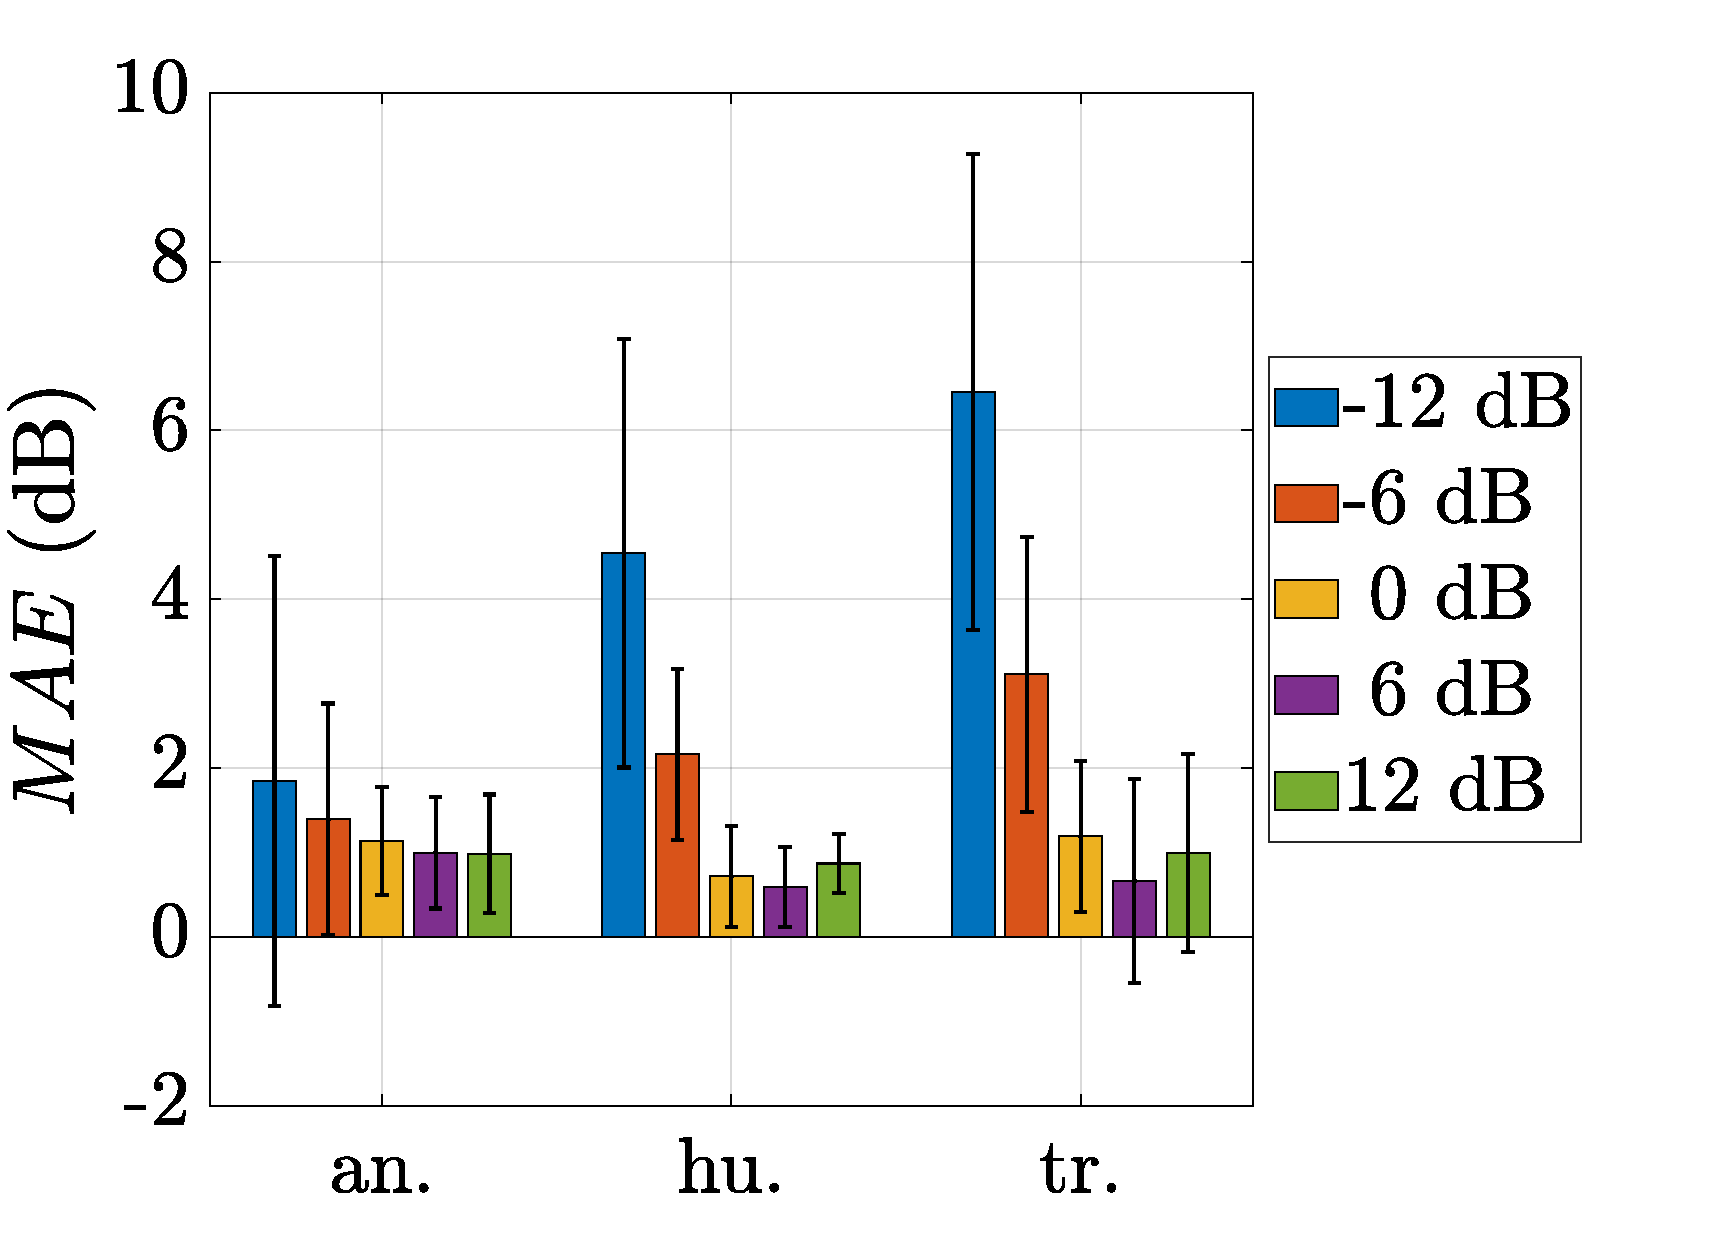
\includegraphics[width=.9\linewidth]{figures/mae_ambiance_bar_ICSV.pdf}
  \caption{ }
  \label{fig:bar_mae}
\end{subfigure}%
\begin{subfigure}{.5\textwidth}
  \centering
  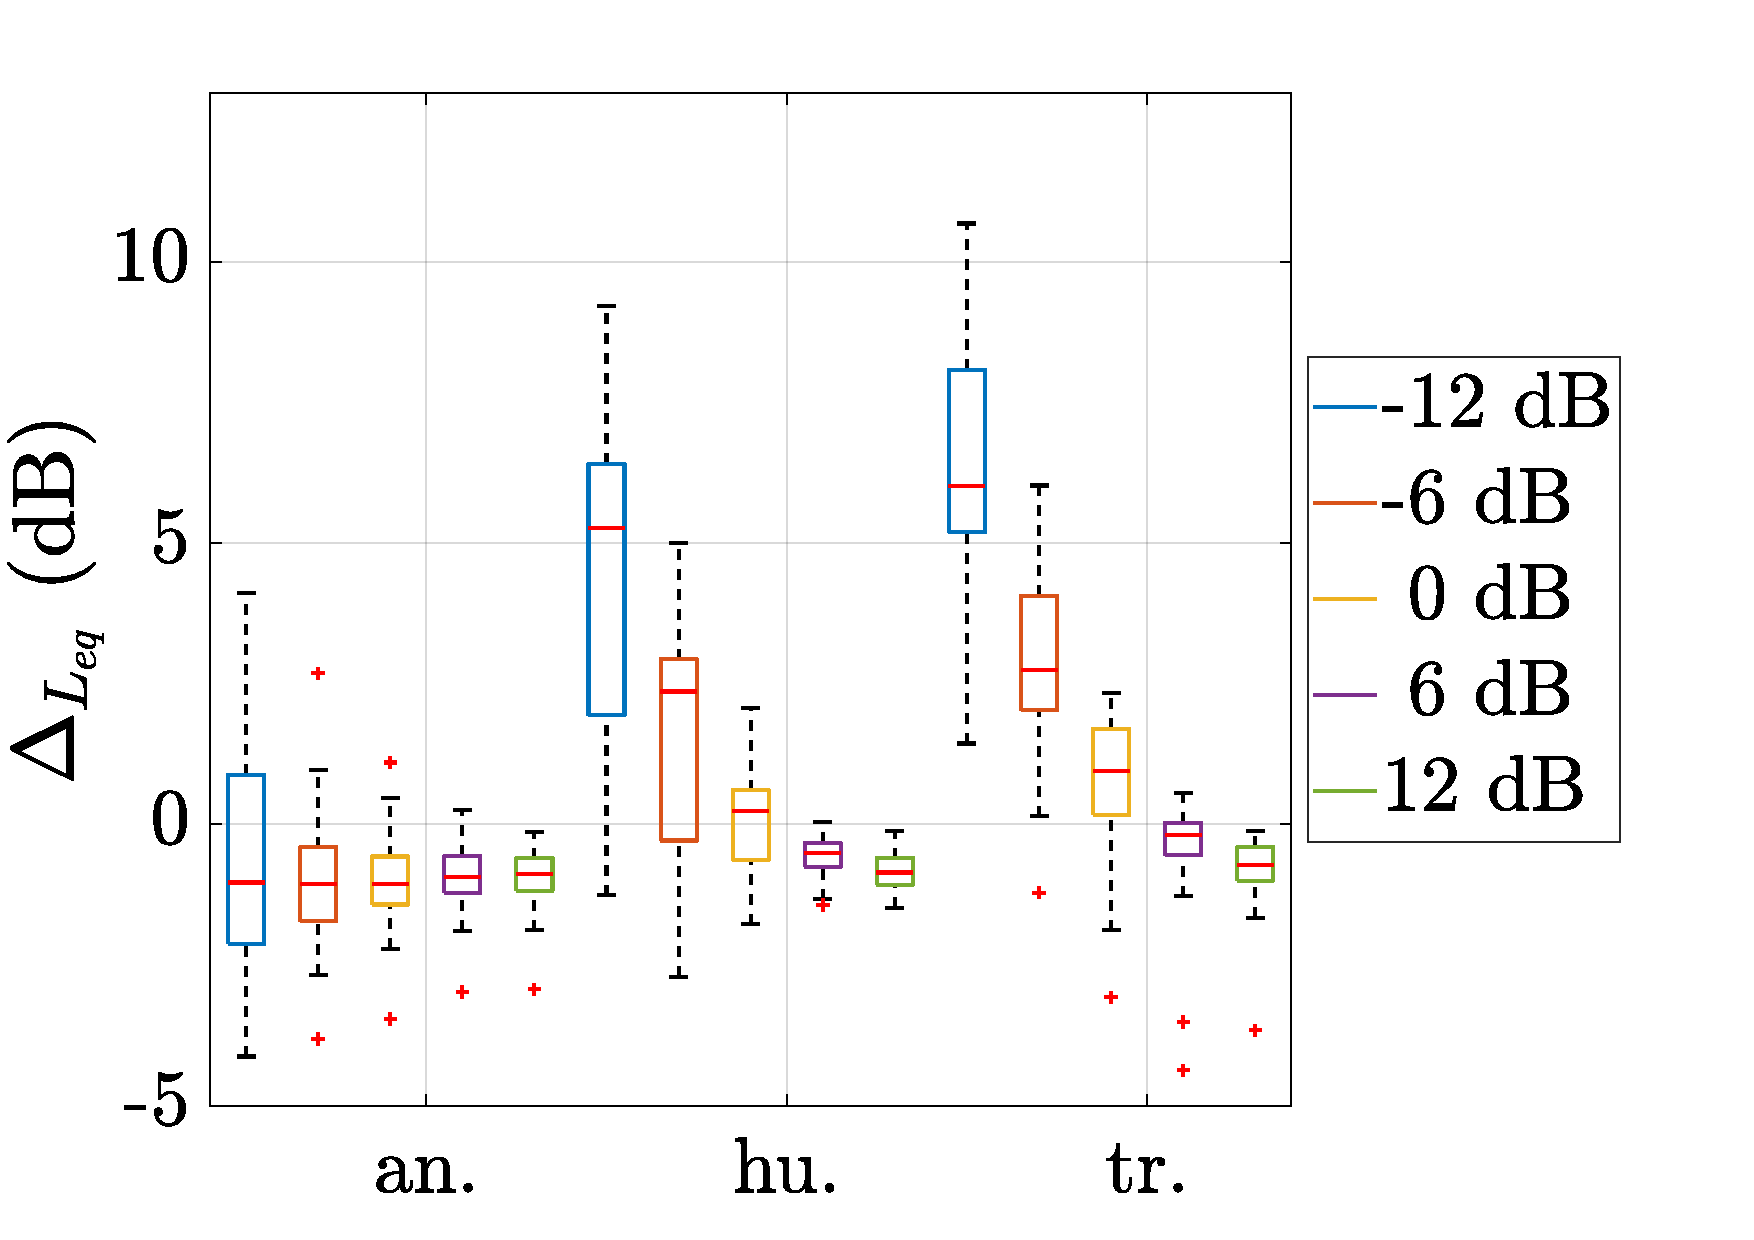
\includegraphics[width=.9\linewidth]{figures/boxplot_amb_nmf_thresholded.pdf}
  \caption{}
  \label{fig:boxplot}
\end{subfigure}
\caption{$MAE$ errors (\subref{fig:bar_mae}) and distribution of relatives error (\subref{fig:boxplot}) on each sub-corpus and $TIR$ value.}
\label{fig:resultat_mae}
\end{figure}

The errors on each sub-corpus and for each $TIR$ value are displayed on Figure \ref{fig:bar_mae}.
The error at $TIR$ = -12 dB, as it is an extreme case where the traffic component is low, are naturally the most important for each sub-corpus with high standard deviation. For \textit{animals} and \textit{transportation}, the $MAE$ errors exceed 3 dB. With the exception of the \textit{transportation} sub-corpus at $TIR = -6$ dB, the rest of the errors are inferior to 3 dB.
The errors for \textit{animals} sub-corpus are lower than the two other sub-corpuses as it contains interfering sound events relative to bird's whistles, in a highest frequencies domain than the traffic spectra, and dog barking, more brief in time.
One observes that the $MAE$ errors for this sub-corpus decrease as the $TIR$ values increase. On the contrary, for \textit{humans} and \textit{transportation} sub-corpus for $TIR \leq 0$ dB, the $MAE$ errors decrease too but increase when $TIR > 0$ dB.
In parallel to the bar distribution of the $MAE$ errors, the distribution of relative errors ($\Delta_{L_{eq}} = \tilde{L}_{eq,traffic}-L_{eq,traffic}$) is added in Figure \ref{fig:boxplot} with boxplots. When $\Delta_{L_{eq}} > 0$, the traffic sound level estimated by TI NMF is over-estimated while it is underestimated when $\Delta_{\tilde{L}_{eq}} < 0$. 
For the \textit{animals} sub-corpus, one notices that TI NMF underestimates the traffic sound level for all $TIR$ values. For the two others sub-corpus, TI NMF mostly  overestimates the traffic sound level when $TIR \leq 0$ dB and then underestimates it when $TIR > 0$ dB.
To better understand the TI NMF behavior, the evolution of the $MAE$ errors according to the threshold and the distance $D(\mathbf{W_0}\vert \vert \mathbf{W})$ shape are displayed in Figure \ref{fig:D_threshold}.

\begin{figure}
\centering
\begin{subfigure}{.5\textwidth}
  \centering
  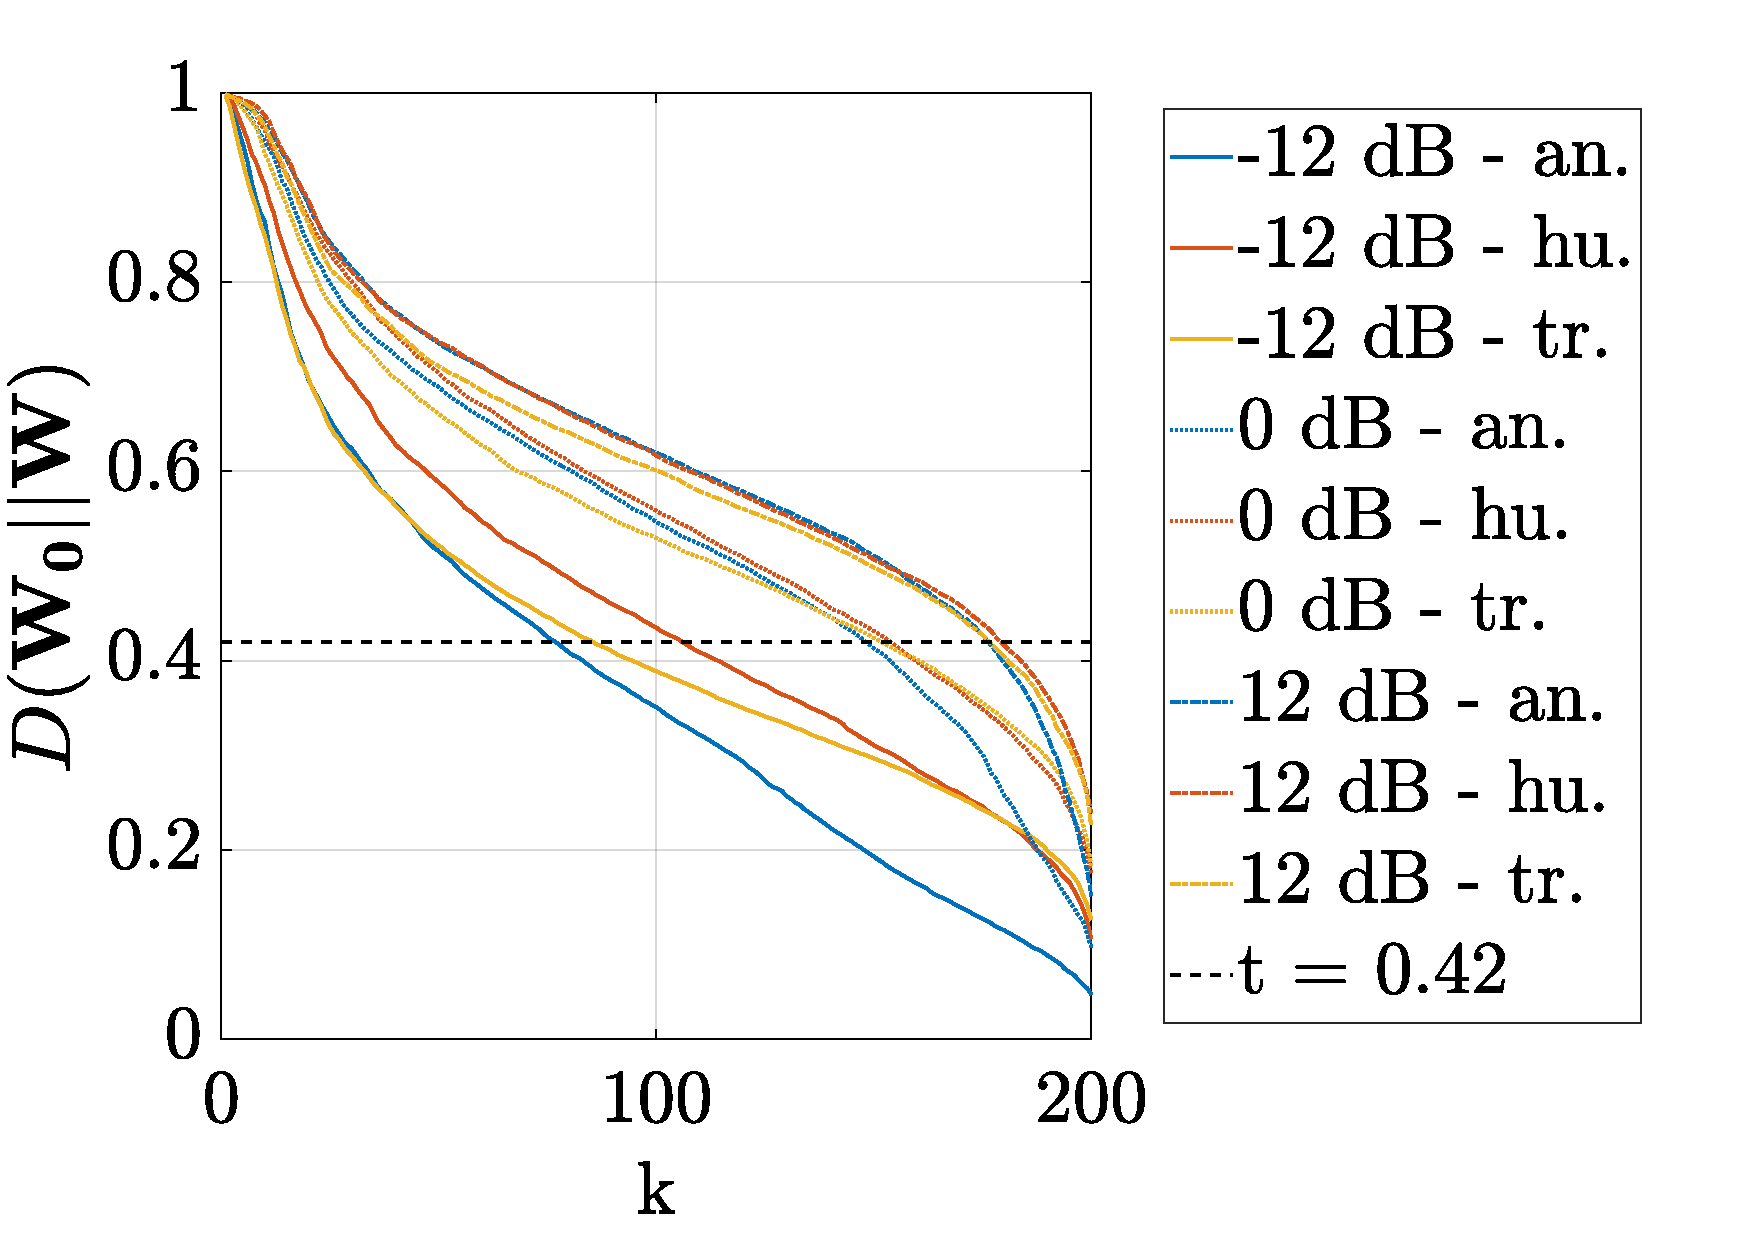
\includegraphics[width=.9\linewidth]{figures/distance_D_ICSV.pdf}
  \caption{ }
  \label{fig:distance_D}
\end{subfigure}%
\begin{subfigure}{.5\textwidth}
  \centering
  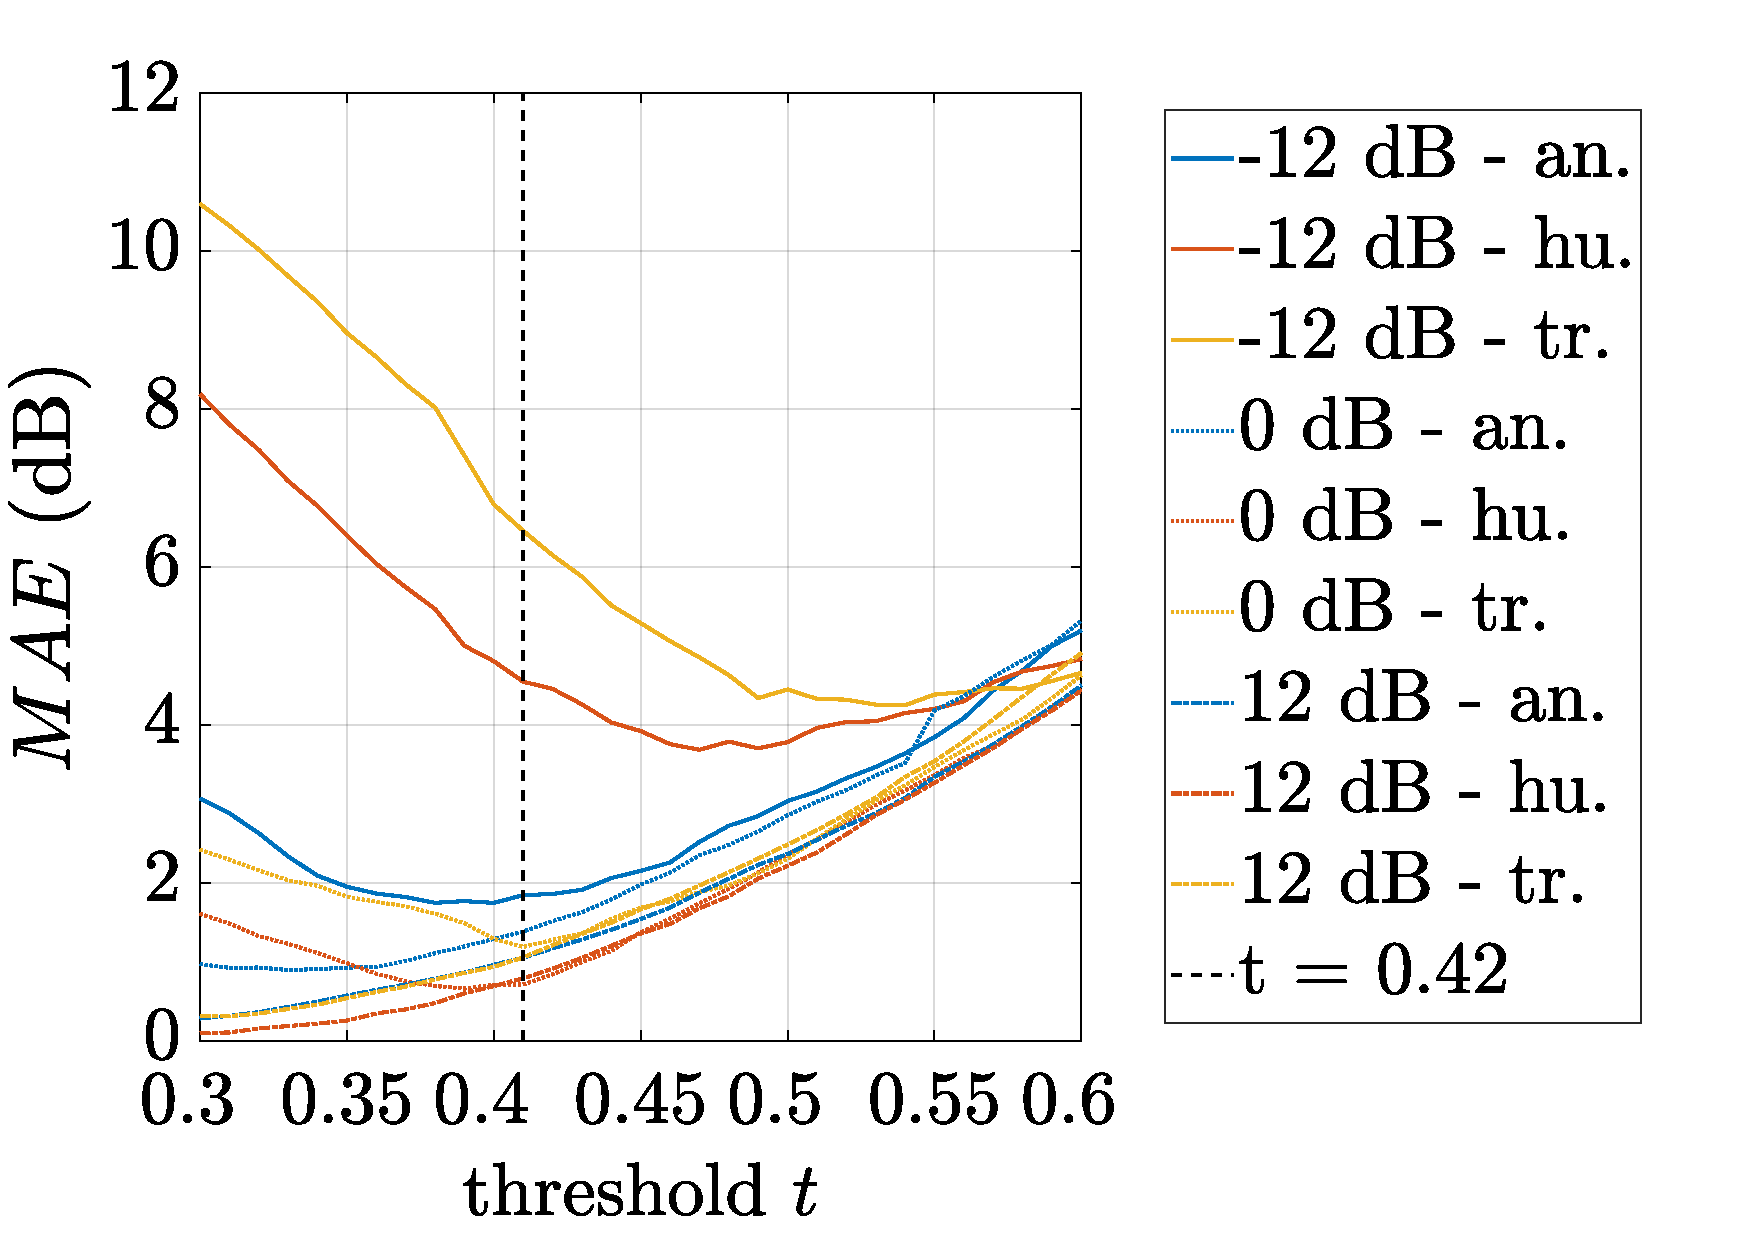
\includegraphics[width=.9\linewidth]{figures/error_mae_amb.pdf}
  \caption{}
  \label{fig:mae_threshold}
\end{subfigure}
\caption{Distances $D(\mathbf{W_0}\Vert \mathbf{W})$ sorted in descend order and $MAE$ errors evolution according threshold values.}
\label{fig:D_threshold}
\end{figure}

In Figure \ref{fig:distance_D}, the distances $D(\mathbf{W_0}\Vert \mathbf{W})$ are sorted in descend order for each $TIR$ values and sub-corpus. Its behavior is variable according to the sub-corpus and the $TIR$ value. 
With the fixed threshold $t = 0.42$, only less than 100 elements from the obtained dictionary $\mathbf{W}$ are considered in $\mathbf{W}_{traffic}$ when $TIR$ = -12 dB. A major part of $\mathbf{W_0}$ diverges from the original traffic spectra to simulate the interfering source. The more the traffic is predominant, the more the number of traffic elements in $\mathbf{W}_{traffic}$ growths. For $TIR = 12$ dB, it is more than 180 elements that are considered. The traffic component is then described by TI NMF with a greater precision. The evolution of $D(\mathbf{W_0}\Vert \mathbf{W})$ is more influenced by the $TIR$ values than by the interfering source as almost the same number of elements are considered in $\mathbf{W}_{traffic}$ whatever the sub-corpus.
TI NMF makes it possible to adapt the dictionary by learning it for each scene. With the fixed threshold it is also a variable number of elements in the $\mathbf{W}_{traffic}$ that are considered,  discarding the other elements that diverge too much from the original traffic spectra on $\mathbf{W_0}$.

Figure \ref{fig:mae_threshold} displays the evolution of the $MAE$ errors according to the threshold and makes it possible to better apprehend the estimation errors. It states the existence of optimal thresholds in each different case. More the $TIR$ value is low, more the threshold has to be high while it has to decrease when the traffic component becomes predominant.
At $TIR$ = -12 dB, for \textit{animals} sub-corpus the optimal threshold is inferior to the fixed threshold $t$ = 0.42 while it is superior for the two other sub-corpuses. As a result, for the first case, TI NMF, with $t$ = 0.42, does not take into account a sufficient number of elements in $\mathbf{W}_{traffic}$ which generate the underestimation of the traffic sound level observed in Figure \ref{fig:boxplot}. On the opposite, as the optimal threshold for the two others classes is higher, TI NMF includes a too important number of elements including the interfering sound classes. This behavior is due to the interfering sound source which is more different with the \textit{animals} sub-corpus than with the \textit{humans} and the \textit{transportation} sub-corpuses. This provokes an overestimation of the traffic sound level.
When the $TIR$ values increase, the traffic component becomes more important in the sound mixtures and in the dictionary $\mathbf{W}$. When $TIR$ = 12 dB, the optimal error is obtained for a lower threshold to almost take into account all the final dictionary $\mathbf{W}$. TI NMF with $t$ = 0.42 discards some traffic spectra which generates the underestimation of the traffic component.  Finally, it has to be reminded that the presence of these sound sources and the $TIR$ values are unknown in an urban context. Despite these different behaviors and performances, TI NMF stays a good approach and makes it possible a compromise to adapt on each case.

\section{Conclusion}

The thresholded initialized Non-negative Matrix Factorization behavior has been studied on urban sound mixtures in order to better apprehend its performances according different urban sound sources dealing with the estimation of the traffic sound level.
With this method, a dictionary $\mathbf{W_0}$ is initialized
with road traffic spectra, updated and the traffic
elements that are similar to the road traffic spectra are then extracted by hard thresholding. 
TI NMF makes it possible to learn a specific dictionary on each scene and to only consider the least divergent part of the dictionary thanks to the selection made during the thresholding step.
The sound database used here is an artificial build-up of a traffic component and different interfering sound classes (\textit{animals}, \textit{humans}, \textit{transportation}) with calibrated sound level in order to propose a controlled framework.
Among the different modalities of the experimental factors, only one combination was retained ($K$ = 200, $w_t$ = 0.5 s, Euclidean distance, $t$ = 0.42). This choice was made in order to reduce the complexity of the study and to propose the most efficient method, whatever the nature of the interference sound source, so as not to add a classification step before.

With this combination, the performances are variable according to the predominance of the traffic and the different interfering sound sources. In the case where the interfering source differs from the road traffic by its spectral and temporal shapes, the errors induced on the estimation of the traffic sound level are low whatever its presence ($MAE <$ 2 dB). These errors tend to decrease with the increase of the traffic presence. In this case, TI NMF tends to underestimate the traffic sound levels because of the fixed threshold that is then too high and does not allow a sufficient number of \textit{traffic} elements to be taken into account in $\mathbf{W}_{traffic}$.
In the case where the spectral shape of the sources are more similar to the road traffic, two types of errors appear. In the case where $TIR \leq 0$ dB, the fixed threshold is considered too low which causes the consideration of interfering elements in the  traffic noise level calculation and thus its overestimation. When $TIR$ is positive, the threshold is now considered as too high which leads to an underestimation of the traffic sound levels.

As a result, the TI NMF performances with a single fixed over the entire corpus make it possible to dispense with the use of a classification step before. It then presents itself as a compromise in its performances according to the predominance of the traffic and its similarity with other interfering sound sources. If the sound scenes are composed of the traffic source and an interfering source, the urban sound environments are the result of the mix of all these sources sometimes emitted simultaneously. Keeping a fixed threshold remains necessary in order to better determine the road traffic sound level in all the cases.

The experimental protocol and the evaluated estimators have been implemented with the Matlab software.
For reproducible purposes, the code is available
online\footnote{\url{https://github.com/jean-remyGloaguen/ICSVnmf2019}}. The evaluation database composed of multiple samples of urban sounds is also made available\footnote{\url{https://zenodo.org/record/1145855}} for the research community with interest in detection, separation and recognition tasks of urban sound sources.

%%This document uses predefined styles to satisfy all the requirements of the 26$^{th}$ International Congress on Sound and Vibration manuscript format. Please while writing your paper do not modify any of the important parameters embedded in this document, such as: fonts, page layout, and style.
%%
%%The most important parameters are hereinafter described: 
%%\begin{itemize}
%%\item Manuscript page size: Letter (215.9 $\times$ 279.4 mm). 
%%\item All manuscript page margins: 20 mm. 
%%\item Basic text font: 12 point Times family font (Times, Times New Roman, etc.). 
%%\item Manuscript Title: 17 points sans-serif font (preferably Helvetica or Arial), in bold. 
%%\item Section titles: 14 point sans-serif font (preferably Helvetica or Arial), in bold. 
%%\item Line spacing: single. 
%%\item Left and right margins: justified. 
%%\item First line of each paragraph: indented by 5 mm. 
%%\end{itemize}
%%
%%
%%\section{First page of the manuscript} 
%%%----------------------------------------------------------------------------------------------
%%
%%
%%Special parts of the manuscript first page include: Congress logo, manuscript title, author names and affiliations and abstract. 
%%
%%
%%\subsection{Manuscript Title} 
%%%----------------------------
%%
%%The title should be typeset using 17 point bold Arial or Helvetica font, with capital letters only. The ``Title'' style has been adjusted to use these values. This style also adjusts vertical spacing
%%above and below the title. If the title is longer than one line, it should be manually broken to equalize line lengths. 
%%
%%
%%\subsection{Author names and affiliations} 
%%%-----------------------------------------
%%
%%Author names should be typeset using 14 point, Times New Roman font, while affiliations should be typeset using 12 point italics Times New Roman font. ``Author'' and``Affiliation'' styles have
%%been defined to use these values. The styles also adjust vertical spacing above and below author and affiliation lines as well as left and right line indentations. 
%%
%%
%%
%%\subsubsection{One author}
%%%-------------------------
%%
%%There is nothing special in case of one author of the manuscript. 
%%
%%
%%\subsubsection{\label{sec:twoauthors} Two or more authors} 
%%%---------------------------------------------------------
%%
%%
%%If there are two or more authors belonging to the same institution, they should be mentioned in one line preceding the affiliation. In this case authors should be separated by commas (,) except for the
%%last author name, which should be preceded by \emph{and}.
%%
%%If there are two or more authors belonging to different institutions, the affiliation should be written for all the authors with a differing institution affiliation. An example of the affiliation style for two or more authors is provided on the first page of this guide.
%%
%%In both cases, there should be only one email address, preferably that of the presenting author. 
%%
%%
%%\subsection{Abstract} 
%%%--------------------
%%
%%The abstract text should be typeset using 11 point Times New Roman font. The abstract text should be separated from the rest of the manuscript with a horizontal line. The ``Abstract'' style has been created to choose this font, to adjust vertical and horizontal spacing around the abstract, and to add the horizontal line.
%%
%%The abstract should be self-contained; therefore, do not refer to the list of references or use acronyms (e.g. SEA for Statistical Energy Analysis). If references cannot be avoided, please put them in full (e.g., ``as described in \textit{Gnus and Gnats of the World}, R. Gneisser, Gnu Publishing, Ltd, 2008''). 
%%
%%The abstract should contain no more than 300 words. 
%%
%%
%%\section{Sections, subsections \dots{}}
%%%----------------------------------------------------------------------------------------------
%%
%%Sections, subsections, and sub subsections should be numbered with Roman numerals. Section, subsection, and sub subsection headings should be typed in sans-serif font (Helvetica, Arial) and left-justified. 
%%
%%Section heading size should be 14 pt. Section headings should be typed using bold face font. The ``Heading 1'' style has been adjusted to follow these rules. 
%% 
%%
%%\subsection{Subsections} 
%%%-----------------------
%%
%%Subsection headings should be typed using bold face font with 12 pt size. The ``Heading 2'' style has been adjusted to follow these rules.
%%
%%
%%\subsubsection{Sub subsection} 
%%%----------------------------
%%
%%Sub subsection headings should be typed using italic font, with 12 pt size. The ``Heading 3'' style has been adjusted to follow these rules.
%%
%%Please do not use deeper section headings than subsubsections. 
%%
%%
%%\section{Mathematical formulas, figures, tables and references}
%%%--------------------------------------------------------------
%%
%%Mathematical formulas, figures, and tables should be separated from the text by a small amount of space below and above them. This space may be used to justify the content vertically on the page. 
%%
%%\subsection{Mathematical formulas}
%%%---------------------------------
%%
%%Mathematical formulas can be placed in the middle of text lines (inline math) or in separate paragraphs. Inline math should be used only for short equations. Please avoid build-up constructions (like fractions, matrices, etc.) in inline math.
%%
%%Long and important mathematical formulas should be placed in separate paragraphs, centered, and with a left-justified number, like the following: 
%%
%%\begin{equation}
%%\label{eq:sum}
%%	\sum_{i=1}^{\infty}\frac{1}{2^{n}}=1
%%\end{equation}
%%
%%
%%Microsoft Word does not provide convenient tools for automatic numeration of equations and making references to them. The ``Equation'' style has been created to make it easier to add a progressive numbering and to produce formulas following the above rules.
%%
%%The style contains two tabulators: a left-justifying tabulator at the left margin and a centering tabulator in the middle of the line. \textbf{To let the formula go in the middle press Ctrl+Tab}.
%%
%%Generally, all displayed formulas should be numbered consecutively, begining with 1. However, only one line of a multi-line formula should be numbered, except when separate references to different lines are necessary. 
%%
%%
%%\subsection{Figures} 
%%%-------------------
%%
%%All illustrations (line drawings, charts, plots, photos, etc.) should be adjusted to provide reasonable trade-offs between resolution and memory usage (the whole paper should be no larger than 2 MB). When scaling an illustration, make sure the font size and line thickness are still large enough to be legible.
%%
%%All illustrations should be centered on the page. However, when there are two or more narrow illustrations, it may be reasonable to put them side-by-side.
%%
%%All illustrations should be captioned \emph{below} the illustration. Captions should be numbered consecutively, centered, and written using a Times family font with point size 11. The ``Caption'' style
%%has been adjusted to follow these rules.
%%
%%\begin{figure}[!htb]
%%	\begin{center}
%%		\includegraphics[width=0.6\textwidth]{immagine.eps}
%%	\caption{\label{fig:immagine} IIAV logo.}
%%	\end{center}
%%\end{figure}
%%
%%
%%\subsection{Tables} 
%%%------------------
%%
%%Tables should be centred on the page. All tables should be captioned \textit{above} the table. Table captions should be numbered consecutively, centred, and written using Times family font with point size 11.
%%
%%\begin{table}[!htb]
%%	\caption{\label{tab:fees} ICSV26 registration fees in Canadian dollars.}
%%	\begin{center}
%%		\begin{tabular}{|c|c|c|c|c|}
%%		\hline
%%		Category & Early OWL                           & Early                              & Late                               & On site \\ 
%%		         &  \footnotesize (paid by 31/12/2018) & \footnotesize (paid by 31/03/2019) & \footnotesize (paid by 31/05/2019) &  \\ 
%%		\hline
%%		IIAV/HELINA Members  & 750  & 900  & 975  & 1050 \\ 
%%		\hline
%%		Non-Members     & 850  & 1000  & 1075  & 1150 \\ 
%%		\hline
%%		Student             & 650  & 750  & 825  & 950 \\ 
%%		\hline
%%		Accompanying person & 100  & 100  & 110  & 125  \\ 
%%		\hline
%%		\end{tabular}
%%	\end{center}
%%\end{table}
%%
%%
%%\subsection{Cross-references} 
%%%----------------------------
%%
%%\subsubsection{Cross-references to equations, figures, \dots{}}
%%%--------------------------------------------------------------
%%
%%
%%When referring to \textbf{equations}, enclose the numbers in parentheses and precede them with ``Eq.'' or ``Eqs.'' Put an unbreakable space between ``Eq.'' and the number (press Ctrl-Shift-Space to insert
%%the unbreakable space). For example, you can refer to Eq (\ref{eq:sum}). You should not begin a sentence with the abbreviation ``Eq.'' or ``Eqs.'' Instead, spell out the word.
%%
%%When referring to figures, precede the number with ``Fig.'' Put an unbreakable space between ``Fig.'' and the number (press Ctrl-Shift-Space to insert the unbreakable space). For example, you can refer to Fig. \ref{fig:immagine}. You should not begin a sentence with the abbreviation ``Fig.'' or ``Figs.'' Instead, spell out the word.
%%
%%When referring to tables, precede the number with the word ``Table.'' Put an unbreakable space between ``Table'' and the number (press Ctrl-Shift-Space to insert the unbreakable space). For example, you
%%can refer to Table \ref{tab:fees}.
%%
%%When referring to sections, subsections, and subsubsections, precede the number with the word ``Section.'' Put an unbreakable space between ``Section'' and the number (press Ctrl-Shift-Space to
%%insert the unbreakable space). For example, you can refer to Section \ref{sec:generalparameters}. Moreover, you can also refer to Section \ref{sec:twoauthors}. 
%%
%%
%%\subsubsection{Cross-references to the literature} 
%%%-------------------------------------------------
%%
%%Use numbers in square brackets to refer to particular positions in the literature. For example, to refer to the first position in the literature list presented at the end of this guide, you should write \cite{Crocker2007}.
%%
%%
%%\section{List of literature references} 
%%%----------------------------------------------------------------------------------------------
%%
%%The heading of the references section should \textit{not} be numbered. The ``RefHeading'' style has been created to be used with the references heading.
%%
%%To save space, references may be set in 10, 11, or 12 point type, with 10 point type being the smallest type that should be used for references. The ``References'' style has been created to be used
%%with the literature list.
%%
%%All references to the literature should appear at the end of the paper. An example of the proper format for references is given at the end of this guide. Please check how to refer to a book, journal paper, or conference paper. The reference number should be typeset as superscript. The title of the journal, book, or conference proceedings should be in italics. The volume number of a journal paper should be typeset using a boldface font.
%%
%%The numbering of references should be in ascending order and should reflect the order of appearance of the references in the text. An example of the proper format for references is given below. 
%%
%%
%%\section{Other important information} 
%%%----------------------------------------------------------------------------------------------
%%
%%
%%\subsection{Number of pages} 
%%%----------------------------------------------------------------------------------------------
%%
%%\textbf{Your manuscript should not exceed the maximum of eight (8) pages.} There is only one exception to the above rule: keynote papers may be up to \textbf{sixteen (16) pages} long.
%%
%%The ICSV26 Organising Committee has the right to \textit{reject papers considered inappropriate} for the proceedings, even if the abstract originally appeared to be acceptable. 
%%
%%
%%\subsection{Submission deadline} 
%%%-------------------------------
%%
%%Peer-reviewed papers are advised to be received as a PDF file no later than \textbf{31 January 2019}. Non-Peer-reviewed papers are advised to be received as a PDF file no later than \textbf{31 March 2019}. In case of any problems in preparing a PDF file, please email the ICSV26 Secretariat at \url{secretariat@icsv26.org}.
%%
%%All papers must be submitted through the congress website: \url{http://www.icsv26.org}. Please login with your email address and password (created when submitting your abstract). Use the ``Remind me my password'' link if you have forgotten your password. Then, follow the instructions on the ``Paper Submission'' subpage. Please note that the online paper submission system only accepts PDF files no larger than 2 MB. In case of any problems during your paper submission, do not hesitate to contact the Congress Secretariat at \url{secretariat@icsv26.org}.
%%
%%
%%\subsection{Presentation} 
%%%------------------------
%%
%%\textbf{Please note that the official language of the ICSV26 Congress  is English.}
%%
%%The presentation time for \textit{keynote papers} will be \textbf{45 minutes}.
%%
%%The presentation time planned for all invited and contributed papers is \textbf{15 minutes}, plus 3 minutes for discussion and 2 minutes for changeover. The session chairman is responsible for keeping to these rules. Please make sure you are able to stay within these limits.
%%
%%Please note that paper presentations will be included in the ICSV26 Scientific Program and full papers in the Congress Proceedings \textbf{only} if at least one registration fee per paper is received by the ICSV26 Secretariat \textbf{before 31 May 2019}. Each registration fee entitles presentation of only one paper; additional presentations are each charged an extra paper fee of CAD 120.
%%
%%
%%
%%----------------------------------------------------------------------------------------------
\begin{small}
\renewcommand\refname{REFERENCES}
\bibliographystyle{icsv_bib}
\bibliography{bibliographie}

\end{small}

\end{document}
